\documentclass[conference]{IEEEtran}
\IEEEoverridecommandlockouts

\usepackage{cite}
\usepackage{amsmath,amssymb,amsfonts}
\usepackage{graphicx}
\usepackage{tikz}
\usetikzlibrary{shapes.geometric, arrows.meta, positioning, fit, backgrounds}
\usepackage{booktabs}
\usepackage{textcomp}
\usepackage{xcolor}
\usepackage{enumitem}

\title{A Machine Learning Framework for Pitting Corrosion Detection in Offshore Infrastructure Using Fused RGB, Thermal, and LiDAR Imagery}

\author{\IEEEauthorblockN{Victor Akhihiero}
\IEEEauthorblockA{\textit{Department of Chemical Engineering} \\
\textit{Universiti Teknologi PETRONAS}\\
victor\_26004080@utp.edu.my
}}

\begin{document}

\maketitle

\begin{abstract}
    Pitting corrosion is among the most dangerous degradation mechanisms affecting offshore infrastructure: it forms concealed, localised cavities that penetrate deep into metal while evading routine visual inspection. In current offshore practice, structural assessment of topside assets and vessel hulls relies predominantly on manual visual inspection. This costly, subjective process requires inspectors to spend prolonged periods in confined spaces. Automated alternatives proposed in research remain largely single-modality, relying chiefly on RGB imagery, which is unreliable in maritime conditions and cannot capture subsurface anomalies or pit geometry. The fusion of RGB, thermal, and laser profilometry has recently proven effective for pitting characterisation, but only in controlled industrial environments and using localised 2D profiling; no existing study extends trimodal fusion to offshore infrastructure. This research builds upon that proven multimodal strategy, extending it to exposed offshore surfaces through drone-deployable LiDAR sensing, using transfer-learned RGB and thermal encoders with a custom fusion design that integrates RGB and thermal features with 3D LiDAR geometry. The methodology encompasses multimodal data acquisition and co-registration, transfer learning of visual backbones, custom fusion design, and systematic evaluation against single- and dual-modality baselines. The expected outcome is a validated trimodal framework for automated pitting detection and severity characterisation, offering improved robustness in offshore conditions alongside quantified evidence of each sensing modality's contribution.
\end{abstract}


\begin{IEEEkeywords}
    Pitting corrosion, offshore infrastructure, sensor fusion, machine learning, transfer learning, RGB-thermal-LiDAR
\end{IEEEkeywords}

\section{Introduction and Background}

Offshore infrastructure, such as oil and gas platforms, floating production storage and offloading (FPSO) vessels, and subsea pipelines, must maintain structural integrity under some of the harshest operating conditions on Earth. These structures are therefore constructed from high-performance metals such as stainless and structural steels, selected for durability and longevity in saline, high-humidity marine environments \cite{dalmora2025methods}. Despite this deliberate material selection, offshore metallic structures remain inherently prone to degradation. The principal cause is corrosion: a chemical and electrochemical process in which metal is progressively oxidised through reactions with its environment \cite{balangao2024corrosion}, substantially accelerated offshore by dissolved salts, oxygen, temperature cycling, and biological activity \cite{dalmora2025methods,bakdash2026analytical}.

Among the different types of corrosion, pitting corrosion is particularly insidious. Unlike uniform corrosion, which thins surfaces evenly and predictably, pitting concentrates attack into small, localised cavities that penetrate deep into the metal while leaving the surrounding surface layer largely intact \cite{balangao2024corrosion}. Because these cavities act as stress concentrators, they can trigger sudden brittle failure \cite{olawole2026advanced}. As a result, a structure may appear sound during routine visual inspection. At the same time, pits propagate toward critical depth, eventually leading to sudden failures like leaks, containment loss, or structural collapse.

The financial and environmental repercussions of corrosion are quantifiable. The direct global cost of corrosion is estimated at approximately USD~2.5 trillion annually, accounting for around 3.4\% of global GDP \cite{kahkesh2025algae, imran2025ship}, rising to beyond USD~4 trillion when costs associated with prevention, control, and productivity losses are included \cite{bakdash2026analytical}. Corrosion contributes to roughly 18\% of significant pipeline incidents, and corrosion-induced failures additionally cause fatalities and environmental pollution \cite{olawole2026advanced, dalmora2025methods}. Fortunately, studies show that effective early detection and maintenance can reduce corrosion-related expenses by an estimated 15--35\% \cite{kahkesh2025algae, imran2025ship}, making early, reliable detection of corrosion paramount for offshore integrity management.

In current offshore practice, structural condition assessment relies heavily on manual visual inspection, with qualified inspectors physically entering tanks and confined spaces—a process that is costly, subjective, and hazardous \cite{soares2023autonomous}. Established non-destructive techniques such as Magnetic Flux Leakage (MFL) and Ultrasonic Testing (UT) are cornerstones of pipeline in-line inspection, but each has inherent limitations (e.g., MFL applies only to ferromagnetic materials), and the data volumes they generate increasingly exceed the capacity of manual analysis \cite{olawole2026advanced}. Research has shifted towards automated detection methods such as RGB imaging, thermal infrared sensing, and 3D laser/LiDAR profiling, combined with machine learning. However, in the offshore domain, these approaches are mostly used separately and are each limited in their capabilities when used alone. Although the fusion of these modalities has proven effective for pitting characterisation, this has so far been demonstrated only in controlled industrial environments, such as boiler tubes, and has not yet been adapted to the offshore domain \cite{zhang2026application}. Indeed, offshore studies achieving high accuracy with single-modality visual methods explicitly identify multimodal fusion as a critical future research direction \cite{imran2025ship}. This proposal aims to address that gap.

\section{Problem Statements}

Three interlocking problems motivate this research:

\textbf{P1 --- Current offshore inspection is manual, and automated alternatives are unreliable.} Offshore structural assessment relies predominantly on manual visual inspection, which is costly, subjective, and hazardous \cite{soares2023autonomous}. Proposed automated visual (RGB) methods degrade under maritime conditions—motion blur, fog, salt spray, surface reflections, and poor lighting in confined spaces \cite{soares2023autonomous, imran2025ship}—and are inherently blind to subsurface corrosion and pit geometry—the maximum depth and volumetric metal loss that maintenance planning relies upon.

\textbf{P2 --- Proven trimodal fusion has not been transitioned offshore.} Fusion of RGB, thermal, and laser profilometry has demonstrated accurate pitting detection and volumetric measurement, but only in controlled industrial environments (boiler tubes) that do not replicate offshore environmental challenges \cite{zhang2026application}.

\textbf{P3 --- No framework exists at the intersection.} No existing study combines RGB, thermal, and LiDAR data to identify and volumetrically measure pitting corrosion on offshore infrastructure, despite explicit calls in the literature for multimodal fusion in offshore inspection \cite{imran2025ship}.

\section{Research Objectives}

Aligned with the problems outlined above, this research addresses the following objectives:

\begin{enumerate}
    \item \label{ro1} Adapt a validated multi-sensor fusion approach that combines RGB, thermal, and LiDAR data streams to detect pitting corrosion in offshore infrastructure.
    \item \label{ro2} Develop a machine learning model using fused modalities and assess its detection performance compared to single- and dual-modality baselines.
    \item \label{ro3} Assess the robustness of the proposed framework by using corrosion datasets that reflect the environmental conditions of offshore infrastructure.
\end{enumerate}

\section{Literature Review}

\subsection{RGB/Visual Image-Based Corrosion Detection}
Deep learning dominates visual corrosion detection. CNN architectures (AlexNet, VGG variants) classify hull-plate corrosion from rust textures and colour irregularities \cite{yao2019artificial}. For pitting specifically, U-Net segmentation has achieved an IoU of 0.9453 for deep-well pit morphology in ship tanks \cite{soares2023autonomous}, while VGG16 transfer learning with an XGBoost head reached 98.47\% accuracy (98.83\% F1) on a 10{,}000-image gas-pipeline dataset \cite{alvani2026corrosion}. Computationally lighter Active Contour approaches attain 98\% classification and 93.83\% segmentation accuracy on ship structures in near real-time, with an execution time of 0.89 seconds \cite{imran2025ship}. However, RGB-only methods perform significantly worse offshore, as metallic reflections and inadequate lighting hinder detection in confined spaces \cite{soares2023autonomous}. Open-sea conditions introduce blur, fog, and salt spray, and trained models generalise poorly across lighting and surface variations \cite{imran2025ship, yao2019artificial}.

\subsection{Thermal/Infrared-Based Detection}
Thermal sensing captures what RGB cannot: subsurface information. Corroded metal retains and releases heat differently from healthy material, producing infrared-detectable temperature variations even beneath paint \cite{zhang2026application}. Short-Wave Infrared (SWIR) imaging with wavelet-based noise removal has achieved 96.2\% detection accuracy for boiler tubes \cite{zhang2026application}. However, thermal corrosion detection still occurs mainly in controlled industrial environments, where it can be affected by dust and water vapour \cite{zhang2026application}. Additionally, no current method adjusts in real time to the changing salinity and temperature conditions offshore.

\subsection{LiDAR and 3D Point Cloud Inspection}
LiDAR and laser profilometry provide geometric dimensions: 3D point cloud pipelines using voxelisation and downsampling quantify maximum and average pit depth and pit volume \cite{zhang2026application, olawole2026advanced}. Coloured point clouds have mapped corrosion across entire vessel hulls \cite{yu2022surface}. The limitations are primarily computational, including high memory usage and power constraints of autonomous platforms, which currently necessitate offline post-processing \cite{olawole2026advanced}.

\subsection{Sensor Fusion and the Research Gap}
Fusion consistently outperforms single-modality detection: RGB+SWIR+laser profilometry achieved 96.2\% accuracy in volumetric pit characterisation of boiler tubes \cite{zhang2026application}; acoustic--image texture fusion reached 98.14\% for pipeline corrosion states \cite{yang2026pipeline}; and GAN-based fusion of magnetic flux leakage and ultrasonic data reconstructs pipeline wall-thickness maps \cite{olawole2026advanced}. However, these domains are boilers, pipelines, and concrete—not offshore structures. Offshore studies remain single- or dual-modality \cite{soares2023autonomous, imran2025ship, yu2022surface}, and Imran et al.\ \cite{imran2025ship} explicitly identify multimodal fusion as the required future direction. This two-layer gap—fusion proven but not offshore, offshore inspection studied but not fused—defines the scope of this research.


\section{Research Design and Methodology}

The research adopts a quantitative, experimental design across four phases, aligned with the research objectives.

\subsection{Phase 1: Data Acquisition and Preparation}
Candidate public corrosion datasets (RGB, thermal, and point cloud) will be identified and evaluated. Where trimodal offshore data is unavailable, complementary strategies will be employed: (i)~cross-domain transfer from industrial multimodal datasets, (ii)~laboratory acquisition of co-registered RGB--thermal--LiDAR imagery of corroded steel specimens, and (iii)~physically informed synthetic data augmentation replicating offshore conditions such as spray, blur, and illumination variation. All modalities will be spatially co-registered and annotated at the pixel/point level for pitting regression.

\subsection{Phase 2: Fusion Framework Adaptation (RO\ref{ro1})}
Rather than designing a fusion architecture from first principles, this research builds on the multi-source fusion methodology validated by Zhang et al.\ \cite{zhang2026application} in industrial boiler environments and adapts it to the offshore domain. Pretrained backbones (e.g., VGG/ResNet-family encoders) will be fine-tuned via transfer learning for the offshore corrosion task across the RGB and thermal streams. The original methodology’s localised laser profilometry will be extended to LiDAR-based sensing to achieve the broader structural coverage required for hulls, tanks, and platform members. Cross-modal registration—aligning 2D RGB and thermal imagery with 3D point cloud data—will be treated as a core technical challenge of the adaptation rather than a routine preprocessing step. Fusion configuration (early, feature-level, and late variants) will be examined empirically as part of the adaptation.

\subsection{Phase 3: Model Development and Evaluation (RO\ref{ro2})}
Models will be developed in Python using established deep learning frameworks, with MATLAB toolboxes (Image Processing, Computer Vision, Lidar, Sensor Fusion) supporting preprocessing and verification. Performance will be assessed using segmentation and detection metrics—such as Intersection over Union (IoU), precision, recall, and F1-score—as well as geometric errors in estimated pit depth and volume where ground truth data exists. The trimodal model will be benchmarked against single-modality (RGB, thermal, LiDAR) and dual-modality baselines under identical training protocols.

\subsection{Phase 4: Robustness Validation (RO\ref{ro3})}
Robustness will be assessed by evaluating the framework under offshore-representative perturbations (illumination shifts, simulated spray/fog, motion blur, sensor noise) and, where feasible, on held-out data from distinct structures to assess generalisation.

\begin{figure}[t]
\centering
\resizebox{0.82\columnwidth}{!}{%
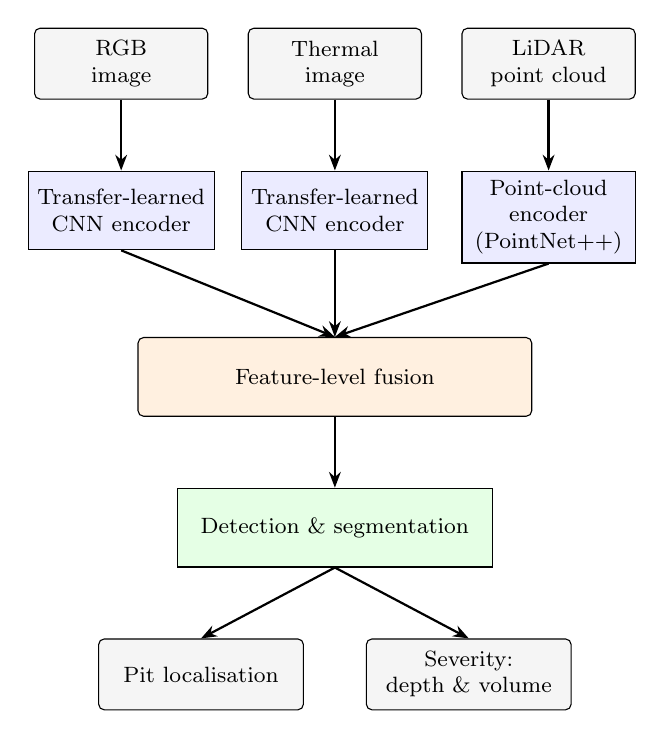
\begin{tikzpicture}[
  font=\footnotesize,
  input/.style={rectangle, rounded corners=2pt, draw=black, fill=gray!8, minimum width=2.2cm, minimum height=0.9cm, align=center},
  enc/.style={rectangle, draw=black, fill=blue!8, minimum width=2.2cm, minimum height=1.0cm, align=center},
  fusion/.style={rectangle, rounded corners=2pt, draw=black, fill=orange!12, minimum width=5.0cm, minimum height=1.0cm, align=center},
  head/.style={rectangle, draw=black, fill=green!10, minimum width=4.0cm, minimum height=1.0cm, align=center},
  outb/.style={rectangle, rounded corners=2pt, draw=black, fill=gray!8, minimum width=2.6cm, minimum height=0.9cm, align=center},
  arr/.style={-{Stealth[length=2mm]}, thick},
]
 
% Input row (top)
\node[input] (rgb) {RGB\\image};
\node[input, right=0.5cm of rgb] (thermal) {Thermal\\image};
\node[input, right=0.5cm of thermal] (lidar) {LiDAR\\point cloud};
 
% Encoder row
\node[enc, below=0.9cm of rgb] (rgbenc) {Transfer-learned\\CNN encoder};
\node[enc, below=0.9cm of thermal] (thermenc) {Transfer-learned\\CNN encoder};
\node[enc, below=0.9cm of lidar] (lidarenc) {Point-cloud\\encoder\\(PointNet++)};
 
% Fusion (full width)
\node[fusion, below=1.1cm of thermenc] (fuse) {Feature-level fusion};
 
% Head
\node[head, below=0.9cm of fuse] (dhead) {Detection \& segmentation};
 
% Outputs (bottom row)
\node[outb, below=0.9cm of dhead, xshift=-1.7cm] (det) {Pit localisation};
\node[outb, below=0.9cm of dhead, xshift=1.7cm] (sev) {Severity:\\depth \& volume};
 
% Arrows inputs -> encoders
\draw[arr] (rgb) -- (rgbenc);
\draw[arr] (thermal) -- (thermenc);
\draw[arr] (lidar) -- (lidarenc);
 
% encoders -> fusion
\draw[arr] (rgbenc.south) -- (fuse.north);
\draw[arr] (thermenc.south) -- (fuse.north);
\draw[arr] (lidarenc.south) -- (fuse.north);
 
% fusion -> head
\draw[arr] (fuse) -- (dhead);
 
% head -> outputs
\draw[arr] (dhead.south) -- (det.north);
\draw[arr] (dhead.south) -- (sev.north);
 
\end{tikzpicture}%
}
\caption{Overview of the proposed RGB--thermal--LiDAR fusion framework for pitting corrosion detection. RGB and thermal streams use transfer-learned CNN encoders; the LiDAR point cloud uses a point-cloud-native encoder. Extracted features are combined in a feature-level fusion module feeding a detection head that outputs pit localisation and severity (depth and volume).}
\label{fig:framework}
\end{figure}

\section{Study Plan}
 
The research spans May 2026 to April 2028 and is structured into six phases, as summarised in Table~\ref{tab:plan}. The literature review represents the longest phase of the project, serving as its foundation. It outlines the current state of the art, identifies the research gap, and results in a comprehensive review paper. It overlaps with the research proposal phase, which formalises the scope and defends it. The programming and tooling phase then builds the technical foundation, progressing from Python and its machine-learning libraries to MATLAB toolboxes for sensor fusion, and finally to C++ for efficient image and point-cloud processing. Dataset acquisition and preprocessing follow, sourcing and co-registering the RGB, thermal, and LiDAR data the model requires. Fusion model development forms the technical core, moving from single-modality baselines to the full trimodal model, then to validation and benchmarking. The final phase covers thesis writing and dissemination. The phases overlap deliberately: programming and tooling proceed alongside dataset acquisition so that implementation skills mature in parallel with data availability.
 
\begin{table}[h]
\caption{Study Plan by Phase (2026--2028)}
\label{tab:plan}
\centering
\small
\begin{tabular}{p{3.6cm}p{4.0cm}}
\toprule
\textbf{Phase / Activity} & \textbf{Period} \\
\midrule
Literature review \& review paper & May 2026 -- Feb 2027 \\
Research proposal \& defence & Jun -- Sep 2026 \\
Programming \& tooling (Python, MATLAB, C++) & Sep 2026 -- Feb 2027 \\
Dataset acquisition \& preprocessing & Nov 2026 -- May 2027 \\
Fusion model development \& experiments & Mar -- Nov 2027 \\
Thesis writing \& dissemination & Oct 2027 -- Apr 2028 \\
\bottomrule
\end{tabular}
\end{table}
 

\section{Key Milestones}
 
Four milestones mark the critical checkpoints of the research, each serving as a deliverable against which progress is assessed (Table~\ref{tab:milestones}). The proposal defence (September 2026) validates the research scope and methodology before substantial implementation begins. The review paper submission in February 2027 consolidates the literature into a peer-reviewed contribution. By November 2027, the fusion model is finalized, marking the completion of the core technical work, after which the results are finalized for the thesis. Finally, the thesis submission and viva (April 2028) serve as the final evaluation of the research.
 
\begin{table}[h]
\caption{Key Milestones}
\label{tab:milestones}
\centering
\small
\begin{tabular}{p{2.0cm}p{5.6cm}}
\toprule
\textbf{Date} & \textbf{Milestone} \\
\midrule
Sep 2026 & Proposal defence \\
Feb 2027 & Review paper submitted \\
Nov 2027 & Fusion model finalised \\
Apr 2028 & Thesis submitted \& viva \\
\bottomrule
\end{tabular}
\end{table}

\section{Expected Outcomes}

The research is expected to deliver:
\begin{enumerate}
    \item A novel machine-learning framework that fuses RGB, thermal, and LiDAR imagery for pitting-corrosion detection in offshore infrastructure—the first at this intersection.
    \item Quantified evidence of each modality's performance contribution through systematic single-, dual-, and trimodal benchmarking.
    \item A co-registered multimodal corrosion dataset and evaluation protocol for reuse by the research community.
    \item Scholarly dissemination comprising a literature review paper and at least one methodology/results publication in venues such as \textit{Ocean Engineering} or \textit{NDT \& E International}.
\end{enumerate}
Practically, the framework aims to enable more reliable, earlier detection of pitting—contributing to the 15--35\% cost reduction achievable through effective early inspection \cite{olawole2026advanced}.


\section{Conclusion}

This proposal has identified a two-layer research gap: trimodal RGB--thermal--LiDAR fusion is proven for pitting characterisation but only in controlled industrial settings, while research in offshore corrosion detection remains restricted to single or dual modalities. The proposed research addresses this intersection through a fused machine learning framework, evaluated rigorously against modality baselines and validated under offshore-representative conditions, within a structured two-year study plan culminating in thesis submission in April 2028.

\bibliographystyle{IEEEtran}
\bibliography{references}

\end{document}